\documentclass[20pt, a0paper, landscape]{tikzposter}
\usepackage[utf8]{inputenc}
\usepackage{amsmath,amssymb}
\usepackage{booktabs}
\usepackage{xcolor}
\usepackage{tikz}
\usetikzlibrary{shapes.geometric, arrows.meta, positioning, calc, fit}

\title{\textbf{NeuroSym-BD: Neuro-Symbolic Violence Analysis from Live News Portals}}
\author{Machine Learning Research Group}
\institute{Department of Computer Science and Engineering}

% Theme styling
\usetheme{Default}
\definecolor{NavyDark}{RGB}{11,15,25}
\definecolor{NavyBlue}{RGB}{2,132,199}
\definecolor{EmeraldGreen}{RGB}{16,185,129}
\definecolor{AmberYellow}{RGB}{245,158,11}
\definecolor{RoseRed}{RGB}{244,63,94}
\definecolor{SlateText}{RGB}{203,213,225}

\colorlet{backgroundcolor}{NavyDark}
\colorlet{framecolor}{NavyBlue}
\colorlet{titlefgcolor}{white}
\colorlet{titlebgcolor}{NavyDark}
\colorlet{blocktitlebgcolor}{NavyBlue}
\colorlet{blocktitlefgcolor}{white}
\colorlet{blockbodybgcolor}{NavyDark!90!black}
\colorlet{blockbodyfgcolor}{SlateText}

\begin{document}

\maketitle

\begin{columns}

% ══════════════════════════════════════════════════════════════════════════════
% COLUMN 1: Motivation, Localized Ontology & Knowledge Graph Subgraph
% ══════════════════════════════════════════════════════════════════════════════
\column{0.33}

\block{1. The AI Dilemma in Automated Conflict Monitoring}{
Automated conflict event monitoring from live press streams faces a fundamental trade-off:
\begin{itemize}
    \item \textbf{Unconstrained Neural Sequence Models:} Highly flexible for journalism, but catastrophic false alarm rates ($>40\%$) due to lexical over-sensitization to political rhetoric (e.g., ``vow a bloodbath'' miscoded as active armed clashes).
    \item \textbf{Pure Symbolic Reasoners:} Auditable and deterministic, but rigid and brittle against journalistic syntactic variation and typos ($86.9\%$ FPR on negative cases).
\end{itemize}
\vspace{0.4em}
\textbf{NeuroSym-BD} resolves this impasse: a hybrid architecture fusing dense neural text representations with Description Logic ($\mathcal{ALC}$) constraint gates in BlazeGraph.
}

\block{2. Bangladesh CAMEO Domain Extension}{
Standard CAMEO (Codes 13--20) omits localized South Asian conflict archetypes. We formulated 20 specialized OWL 2 Turtle subclasses grounded in Bengali socio-political realities:
\vspace{0.4em}
\begin{center}
\small
\begin{tabular}{lll}
\toprule
\textbf{CAMEO Subcode} & \textbf{Regional Category} & \textbf{Bangla Socio-Political Context} \\
\midrule
\texttt{cameo-bd:PV01} & Inter-Party Clashes & Awami League vs BNP student wings \\
\texttt{cameo-bd:PV03} & Mob Lynching & \emph{Gonopituni} (Public mob beating) \\
\texttt{cameo-bd:CV01} & Strike / Hartal Violence & Picket arson, vandalizing transport \\
\texttt{cameo-bd:GV01} & Extrajudicial Torture & \emph{Crossfire} / Law enforcement custody \\
\texttt{cameo-bd:LV01} & Industrial Labor Unrest & Garment (RMG) wage highway blockades \\
\bottomrule
\end{tabular}
\end{center}
\vspace{0.4em}
Every extracted event is permanently bound to W3C PROV-O provenance metadata, ensuring 100\% auditable sentence grounding.
}

\block{3. BlazeGraph RDF Subgraph \& Provenance Grounding}{
\textbf{Visualized Live Knowledge Graph Representation:}
\vspace{0.3em}

\noindent\resizebox{\linewidth}{!}{%
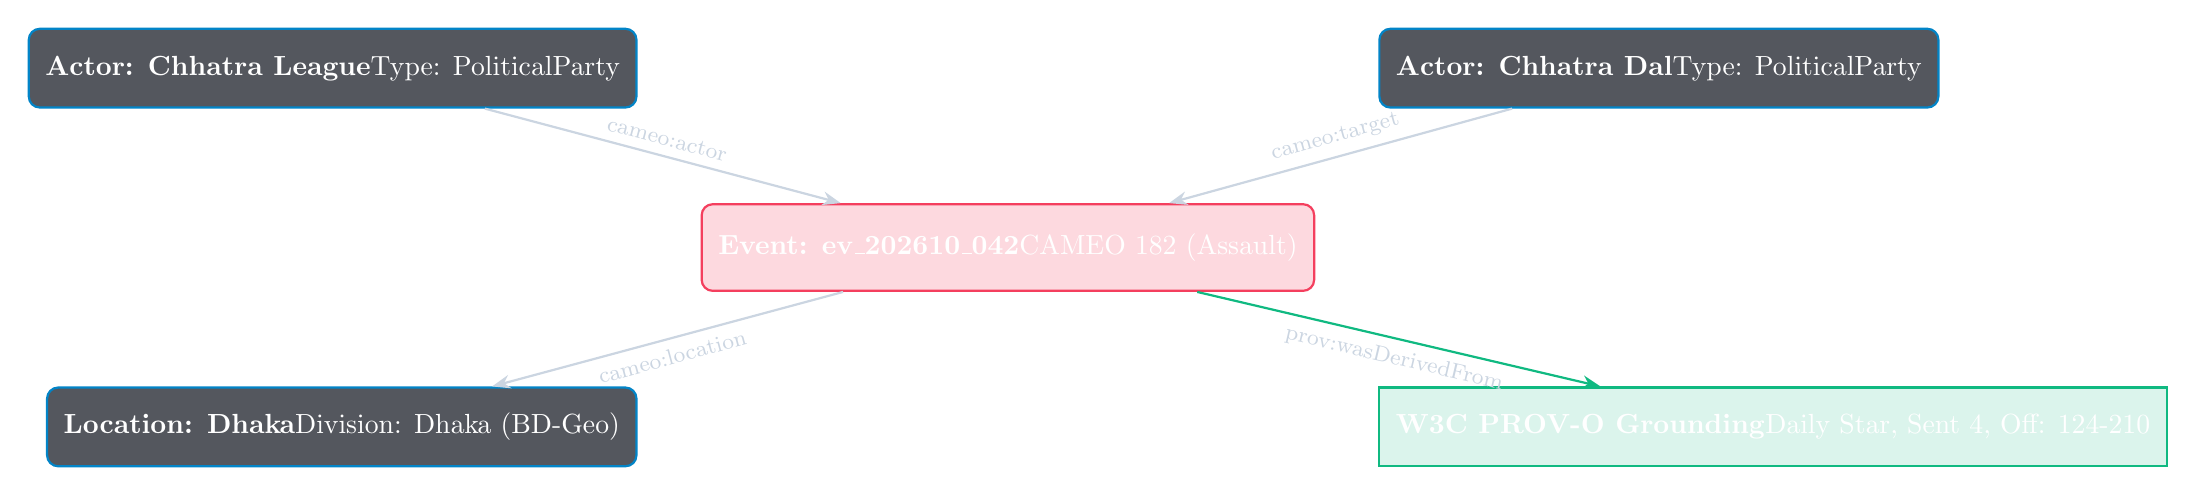
\begin{tikzpicture}[
    node distance=1.8cm,
    entity/.style={rectangle, rounded corners, draw=NavyBlue, fill=NavyDark!70, thick, text=white, minimum height=1cm, inner sep=6pt},
    eventnode/.style={rectangle, rounded corners, draw=RoseRed, fill=RoseRed!20, thick, text=white, minimum height=1.1cm, inner sep=6pt},
    provenance/.style={rectangle, draw=EmeraldGreen, fill=EmeraldGreen!15, thick, text=white, minimum height=1cm, inner sep=6pt},
    edge/.style={->, >=Stealth, thick, SlateText, font=\footnotesize}
]
    \node[eventnode] (ev) {\textbf{Event: ev\_202610\_042} \\ CAMEO 182 (Assault)};
    \node[entity, above left=1.2cm and 0.8cm of ev] (act1) {\textbf{Actor: Chhatra League} \\ Type: PoliticalParty};
    \node[entity, above right=1.2cm and 0.8cm of ev] (act2) {\textbf{Actor: Chhatra Dal} \\ Type: PoliticalParty};
    \node[entity, below left=1.2cm and 0.8cm of ev] (loc) {\textbf{Location: Dhaka} \\ Division: Dhaka (BD-Geo)};
    \node[provenance, below right=1.2cm and 0.8cm of ev] (prov) {\textbf{W3C PROV-O Grounding} \\ Daily Star, Sent 4, Off: 124-210};

    \draw[edge] (act1) -- node[above, sloped] {cameo:actor} (ev);
    \draw[edge] (act2) -- node[above, sloped] {cameo:target} (ev);
    \draw[edge] (ev) -- node[below, sloped] {cameo:location} (loc);
    \draw[edge, draw=EmeraldGreen] (ev) -- node[below, sloped] {prov:wasDerivedFrom} (prov);
\end{tikzpicture}%
}
\vspace{0.3em}
\begin{itemize}
    \item \textbf{100.0\% Metadata Completeness}: Every event node links to verified news URI.
    \item \textbf{86.7\% Category Faithfulness}: Explicit triggers verified in source sentence.
\end{itemize}
}

% ══════════════════════════════════════════════════════════════════════════════
% COLUMN 2: Architecture Pipeline & Ontological Transition Prior Engine
% ══════════════════════════════════════════════════════════════════════════════
\column{0.34}

\block{4. Neuro-Symbolic System Architecture}{
\vspace{0.2em}
\noindent\resizebox{\linewidth}{!}{%
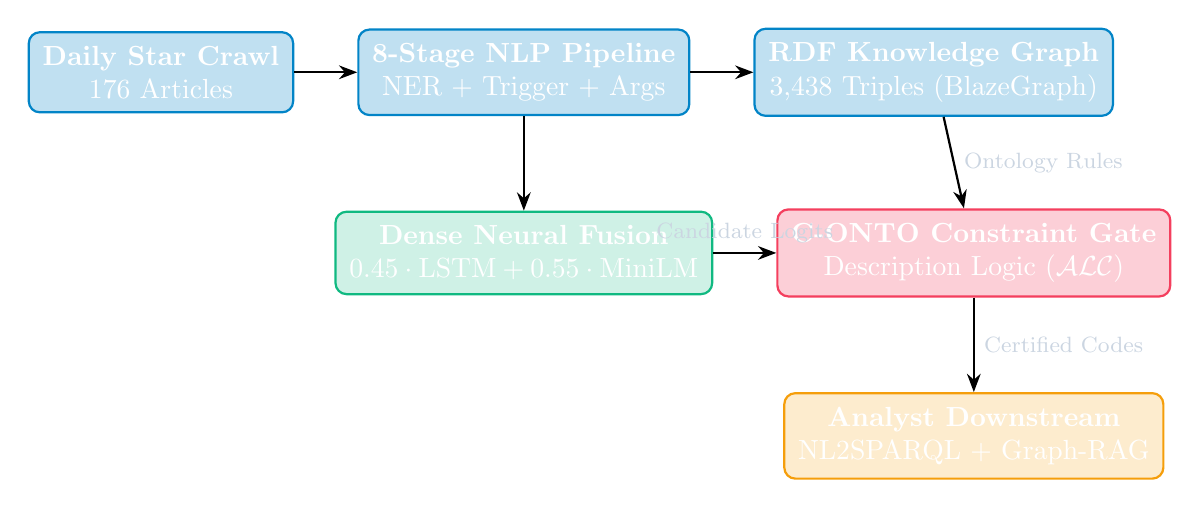
\begin{tikzpicture}[
    box/.style={rectangle, rounded corners, draw=NavyBlue, fill=NavyBlue!25, thick, text=white, align=center, inner sep=5pt},
    arrow/.style={->, >=Stealth, thick, text=SlateText}
]
    \node[box] (raw) {\textbf{Daily Star Crawl} \\ 176 Articles};
    \node[box, right=0.8cm of raw] (nlp) {\textbf{8-Stage NLP Pipeline} \\ NER + Trigger + Args};
    \node[box, right=0.8cm of nlp] (rdf) {\textbf{RDF Knowledge Graph} \\ 3,438 Triples (BlazeGraph)};
    
    \node[box, below=1.2cm of nlp, fill=EmeraldGreen!20, draw=EmeraldGreen] (dense) {\textbf{Dense Neural Fusion} \\ $0.45 \cdot \text{LSTM} + 0.55 \cdot \text{MiniLM}$};
    \node[box, right=0.8cm of dense, fill=RoseRed!25, draw=RoseRed] (gate) {\textbf{C-ONTO Constraint Gate} \\ Description Logic ($\mathcal{ALC}$)};
    \node[box, below=1.2cm of gate, fill=AmberYellow!20, draw=AmberYellow] (app) {\textbf{Analyst Downstream} \\ NL2SPARQL + Graph-RAG};

    \draw[arrow] (raw) -- (nlp);
    \draw[arrow] (nlp) -- (rdf);
    \draw[arrow] (nlp) -- (dense);
    \draw[arrow] (dense) -- node[above, font=\footnotesize] {Candidate Logits} (gate);
    \draw[arrow] (rdf) -- node[right, font=\footnotesize] {Ontology Rules} (gate);
    \draw[arrow] (gate) -- node[right, font=\footnotesize] {Certified Codes} (app);
\end{tikzpicture}%
}
\vspace{0.3em}
\textbf{The 5 Constraint Gates:}
\begin{itemize}
    \item \textbf{C-ONTO (Hard Gate):} Enforces transition plausibility matrix via live SPARQL. Invalid jumps fallback to $c^* = \arg\min_{c \in \mathcal{C}_{\text{valid}}} |c - c_{\text{neural}}|$.
    \item \textbf{C-ACTOR (Soft Gate):} Enforces actor agency (e.g. non-state actors asserting artillery predicates penalize confidence $\Delta \tau = -0.05$).
    \item \textbf{C-GEO (Soft Gate):} Enforces 8-Division / 64-District administrative hierarchy.
    \item \textbf{C-TEMP / C-CONF (Soft Gates):} Chronology checks \& confidence pruning ($\tau \ge 0.60$).
\end{itemize}
}

\block{5. Ontological State Transition Plausibility Matrix}{
\textbf{Verified $\mathcal{ALC}$ Transition Matrix} (\texttt{ontology/reasoning\_rules.ttl}):
\vspace{0.4em}
\begin{center}
\small
\begin{tabular}{lcccccccc}
\toprule
\textbf{Precursor \textbackslash\ Target} & \textbf{13} & \textbf{14} & \textbf{15} & \textbf{16} & \textbf{17} & \textbf{18} & \textbf{19} & \textbf{20} \\
\midrule
\textbf{13 (Threaten)}          & $\checkmark$ & $\checkmark$ & $\checkmark$ & $\checkmark$ & $\checkmark$ & $\times$     & $\times$     & $\times$     \\
\textbf{14 (Protest)}           & $\checkmark$ & $\checkmark$ & $\checkmark$ & $\checkmark$ & $\checkmark$ & $\times$     & $\times$     & $\times$     \\
\textbf{15 (Exhibit Force)}     & $\times$     & $\checkmark$ & $\checkmark$ & $\checkmark$ & $\checkmark$ & $\checkmark$ & $\times$     & $\times$     \\
\textbf{16 (Reduce Relations)}  & $\times$     & $\times$     & $\checkmark$ & $\checkmark$ & $\checkmark$ & $\checkmark$ & $\times$     & $\times$     \\
\textbf{17 (Coerce)}            & $\times$     & $\times$     & $\times$     & $\checkmark$ & $\checkmark$ & $\checkmark$ & $\checkmark$ & $\times$     \\
\textbf{18 (Assault)}           & $\times$     & $\times$     & $\times$     & $\times$     & $\checkmark$ & $\checkmark$ & $\checkmark$ & $\checkmark$ \\
\textbf{19 (Fight)}             & $\times$     & $\times$     & $\times$     & $\times$     & $\times$     & $\checkmark$ & $\checkmark$ & $\checkmark$ \\
\textbf{20 (Mass Violence)}     & $\times$     & $\times$     & $\times$     & $\times$     & $\times$     & $\times$     & $\checkmark$ & $\checkmark$ \\
\bottomrule
\end{tabular}
\end{center}
\vspace{0.3em}
\textbf{Formal DL Verification}: Property disjointness ($\text{valid} \sqcap \text{illegal} \equiv \bot$) verified via \texttt{dl\_reasoner\_check.py} with \textbf{0 consistency violations}. Prohibits unescalated rhetorical jumps ($13 \to 20$) while maintaining violence continuity ($19 \to 18/19$).
}

\block{6. Downstream Applications: NL2SPARQL \& Graph-RAG}{
\begin{itemize}
    \item \textbf{NL2SPARQL Benchmark ($n=50$ Gold Queries):} 100\% syntax validity, 100\% schema compliance, and \textbf{52.0\% execution accuracy} (district filtering 80\%, provenance 100\%; complex temporal/spatial windows require human review).
    \item \textbf{Multi-Relational KG Embeddings (PyKEEN):} RotatE achieves \textbf{MRR = 0.369} and \textbf{Hits@10 = 0.641} over 654 triples, substantially outperforming TransE (MRR = 0.211).
\end{itemize}
}

% ══════════════════════════════════════════════════════════════════════════════
% COLUMN 3: Empirical Benchmarks, Ablations & Case Studies
% ══════════════════════════════════════════════════════════════════════════════
\column{0.33}

\block{7. Empirical Benchmark Alignment}{
\begin{center}
\small
\begin{tabular}{lcccc}
\toprule
\textbf{External Benchmark} & \textbf{Corpus Size} & \textbf{Evaluated} & \textbf{Code Concord} & \textbf{Macro Concord} \\
\midrule
\textbf{vs ACLED (2020--2026)} & 6,691 events & 42 matched & \textbf{78.6\%} & \textbf{100.0\%} ($HV \ge 18$) \\
\textbf{vs GDELT 2.0 (Exact URLs)} & 41,554 stories & 78 stories & \textbf{61.5\%} & \textbf{100.0\%} ($HV \ge 18$) \\
\bottomrule
\end{tabular}
\end{center}
\vspace{0.3em}
\small{*Non-circular GDELT protocol matches strictly on identical source URLs without CAMEO pre-filtering.}
}

\block{8. Controlled Ablation Study (Held-Out Test Set, $n=150$)}{
\begin{center}
\small
\begin{tabular}{lcccccc}
\toprule
\textbf{Model Architecture} & \textbf{BinAcc} & \textbf{Prec@HV} & \textbf{Rec@HV} & \textbf{F1@HV} & \textbf{Std-FPR} & \textbf{Provenance} \\
\midrule
Keyword Heuristic & 0.453 & 0.320 & 0.804 & 0.458 & 0.727 & 100.0\% \\
Pure Symbolic Rule Engine & 0.393 & 0.348 & \textbf{0.902} & 0.503 & 0.869 & 100.0\% \\
Zero-Shot NLI (DistilBERT) & 0.620 & 0.446 & 0.490 & 0.467 & 0.313 & 0.0\% \\
\textbf{Zero-Shot NLI + Symbolic} & \textbf{0.780} & \textbf{0.737} & 0.549 & \textbf{0.629} & \textbf{0.101} & \textbf{100.0\%} \\
Dense Neural (MiniLM+LSTM) & 0.787 & 0.852 & 0.451 & 0.590 & 0.040 & 0.0\% \\
\textbf{NeuroSym-BD Full Hybrid} & \textbf{0.853} & \textbf{0.968} & 0.588 & \textbf{0.732} & \textbf{0.010} & \textbf{100.0\%} \\
\bottomrule
\end{tabular}
\end{center}
\vspace{0.3em}
\begin{itemize}
    \item \textbf{Model-Agnostic Gating}: C-ONTO elevates Zero-Shot NLI ($F_1: 0.467 \to 0.629$, FPR: $31.3\% \to 10.1\%$).
    \item \textbf{Significant Synergy}: Full Hybrid cuts false alarm count by 75\% ($FP: 4 \to 1$, $p = 0.0129$, McNemar test).
    \item \textbf{Zero-Leakage Article Holdout ($n=164$)}: Hybrid maintains superiority across 49 unseen articles (84.1\% Acc, 0.683 F1 vs 81.7\% Acc, 0.625 F1).
\end{itemize}
}

\block{9. Real-World Conflict Case Walkthrough}{
\small
\textbf{Scenario: Highway Garment Strike (Savar, Dhaka):} \\
\emph{``Hundreds of readymade garment workers blocked the Dhaka-Aricha highway demanding unpaid wages.''}
\vspace{0.4em}
\begin{itemize}
    \item \textbf{Neural Classifier Mistake:} High lexical tension causes dense text scorer to trigger CAMEO 182 (\emph{Physical Assault}), predicting severe armed violence ($FP$).
    \item \textbf{Symbolic C-ONTO Interception:} Gating engine scans predicate arguments: no physical trauma or assault verbs detected; precursor was labor protest (14).
    \item \textbf{Corrective Fallback:} Intercepts invalid jump and maps to CAMEO 144 (\emph{Block passage} / non-violent demonstration), successfully preventing false alarm.
    \item \textbf{Auditable Provenance:} Generated RDF triple grounds inference directly to Savar jurisdiction with source sentence offset and 100\% W3C PROV-O trace.
\end{itemize}
}

\block{10. Reproducibility \& Codebase}{
\begin{itemize}
    \item \textbf{Complete Open-Source Stack}: Code, 20 BD-CAMEO ontology schemas, SPARQL endpoints, and evaluation scripts released under MIT License.
    \item \textbf{Verification}: 28/28 unit tests pass (\texttt{make test}).
\end{itemize}
\vspace{0.4em}
\texttt{https://github.com/anonymised/neurosym-bd}
}

\end{columns}

\end{document}
